\question{Переходы внутренних электронов в атомах. Рентгеновские спектры. 
Закон Мозли. Эффект Оже.}

\subquestion{Переходы внутренних электронов в атомах}
Рассмотрим переходы связанные с изменением состояния внутренних атомных 
электронов. В этом случае возникает характеристическое рентгеновское 
излучение. 

В отличие от оптических спектров, которые являются индивидуальными для 
каждого конкретного элемента, рентгеновские спектры различных элементов 
похожи друг на друга. Это связано с тем, что изменение количества 
электронов во внешней атомной оболочке кардинальным образом сказывается на 
энергетическом спектре системы. В то же время внутренние атомные электроны 
находятся, прежде всего, в потенциале, создаваемом атомным ядром, который 
лишь частично экранируется электронной оболочкой. Поэтому их энергия 
плавно меняется с изменением заряда ядра, однако качественной перестройки 
спектра не происходит.

Тот факт что электроны, находящиеся на внутренних атомных оболочках, 
<<чувствуют>>, прежде всего, кулоновский потенциал атомного ядра -- 
\( Ze^2 / r \), а учёт межэлектронного взаимодействия может быть сделан в 
рамках теории возмущений, означает возможность описания внутренних атомных 
электронов в одночастичном приближении, причём их волновые функции и 
положение энергетического являются водородоподобными.

\subquestion{Рентгеновские спектры}
Рентгеновские спектры можно разделить на два подвида:
\begin{enumerate}
	\item Тормозное излучение
	\item Характеристическое излучение
\end{enumerate}

\emph{Тормозное излучение} наблюдается при небольших энергиях электрона, 
имеет сплошной спектр и не зависит от материала антикатода.

\emph{Характеристическое излучение} наблюдается при больших значениях 
энергии (достаточные для вырывания электрона из внутренней оболочки атома), 
имеет линейчатый спектр и зависит от материала антикатода. 

Особенности характеристических спектров:
\begin{enumerate}
	\item рентгеновский характеристический спектр различных элементов 
		отличается простотой и однообразностью в отличии от оптических и 
		линейчатых спектров;
	\item с увеличением атомного номера спектры смещаются в сторону коротких 
		волн;
	\item характеристические спектры различных элементов имеют однотипный 
		характер. Это объясняется тем, что характеристические спектры 
		образуются при переходах электрона во внутренних оболочках, а 
		внутренние оболочки различных элементов имеют схожее строение.
	\item характеристические спектры состоят из серий. Серии обозначаются также 
		как и внутренние оболочки атомов: \( K, L, M\); каждая серия состоит 
		из небольшого количества линий: 
		\( K_\alpha, K_\beta, ...; L_\alpha, L_\beta, L_\gamma\)
\end{enumerate}

Схема возникновения рентгеновского характеристического спектра:

\begin{figure}[h!]
    \center
    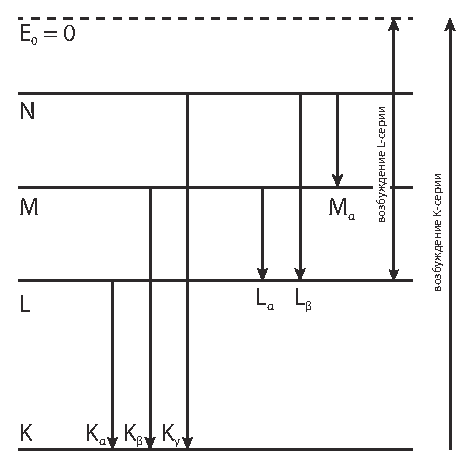
\includegraphics[width=.47\textwidth]{14_01}
\end{figure}

Если вырвать один из двух электронов в \( K \) слое, то освобожденное место 
может быть занято электроном из более высшей оболочки \( L, M, ... \). Так 
возникает \( K \)-серия. Серия \( K \) обязательно сопровождается остальными 
сериями, так как в высших слоях также освобождаются места для переходов 
электронов с ещё более высших слоёв.

Особенность поглощения характеристического излучения состоит в том, что спектр 
поглощения не совпадает со спектром испускания. Спектр поглощения представляет 
собой широкие полосы поглощения с резкими краями.

\begin{figure}[h!]
    \center
    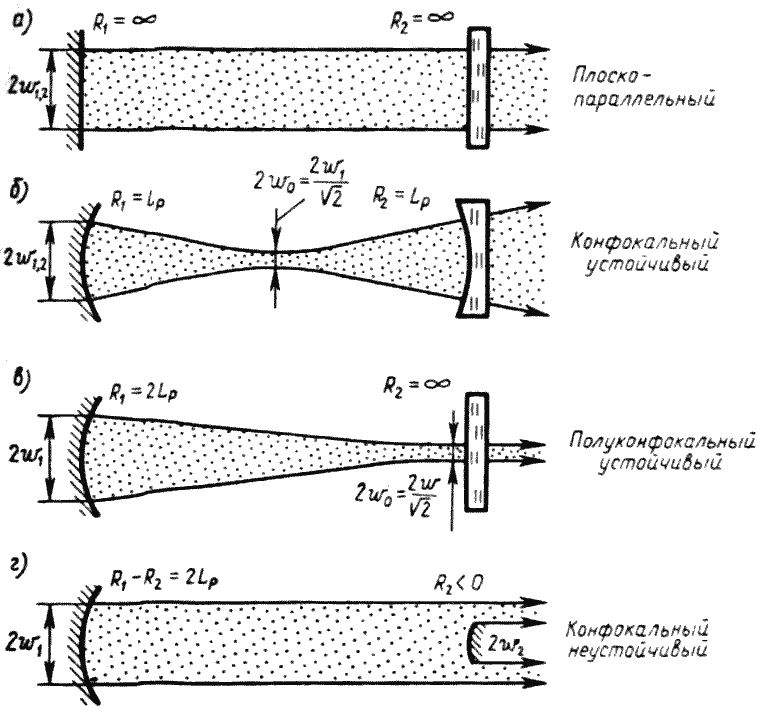
\includegraphics[width=.47\textwidth]{14_02}
\end{figure}

Такая особенность поглощения рентгеновского излучения объясняется тем что при 
малых длинах волн (или высоких энергиях) возбуждаются все серии от \( K \) до ... 
При увеличении длины волны от \( \lambda \) до \( \lambda_k \) (что соответствует 
уменьшению энергии падающего излучения) происходит прекращение возбуждения 
\( K \)-серии появляется так называемый \( K \)-край полосы поглощения. При 
дальнейшем увеличении \( \lambda \) (или уменьшении энергии) на кривой поглощения 
появляется \( L \)-край состоящий из трёх зубцов. Появление зубчиков связано с 
тонкой структурой рентгеновских спектров.

\[ K: n = 1, l = 0, S = \frac{1}{2}, J = \frac{1}{2} \]
\[ 
	L: n = 2, \left. \begin{array}
		l = 0, J = \frac{1}{2} \\
		l = 1, J = \frac{3}{2}, \frac{1}{2}
	\end{array} \right\} \text{ 3 зубчика }
\]
\[ M: \text{ 5 зубчиков }\]

\subquestion{Закон Мозли}
Закон Мозли -- закон, связывающий частоту спектральных линий 
характеристического рентгеновского излучения атома химического 
элемента с его порядковым номером. Экспериментально установлен 
английским физиком Генри Мозли в 1913 году.

Корень из частоты излучения является линейной функцией заряда атомного ядра.
\[ \sqrt\omega \sim R(Z-\sigma) \]

В соответствии с Законом Мозли, рентгеновские характеристические 
спектры не обнаруживают периодических закономерностей, присущих 
оптическим спектрам. Это указывает на то, что проявляющиеся в 
характеристических рентгеновских спектрах внутренние электронные оболочки 
атомов всех элементов имеют аналогичное строение.

\[
	\omega_{k\alpha} = R(z-\sigma_k)^2(\frac{1}{1^2} - \frac{1}{2^2}) =
	\frac{3}{4}R(z-\sigma_k)^2
\]
\[
	\omega_{k\beta} = R(z-\sigma_k)^2(\frac{1}{1^2} - \frac{1}{3^2}) = 
	\frac{8}{9}R(z-\sigma_k)^2
\]
\[ 
	\omega = R\left( \frac{(z-\sigma_{n1})^2}{n^2_1} -
	\frac{(z-\sigma_{n2})^2}{n^2_2}\right)
\]

\subquestion{Эффект Оже}
Падающее на вещество рентгеновское излучение выбивает один из внутренних 
электронов при этом на внутренней оболочке образуется вакансия. Такое 
состояние атома неустойчиво и поэтому атом стремится минимизировать энергию 
за счёт заполнения вакансии электрона с одного из выше лежащих уровней. В 
результате этого перехода выделяется некоторая энергия -- она может быть 
испущена в виде кванта характерного излучения либо передана третьему электрону, 
который при этом вынужденно покидает атом. Второй эффект называется -- 
Эффект Оже. Он характерен для лёгких атомов и энергии связи меньше чем 1 КэВ. 
В результате атом становится дважды ионизированным. 

\begin{figure}[h!]
    \center
    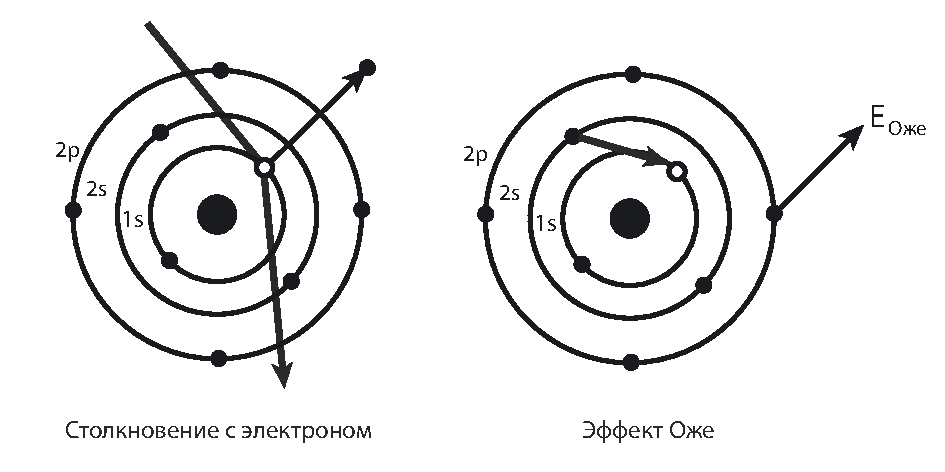
\includegraphics[width=.47\textwidth]{14_03}
\end{figure}

\newpage
